\begin{spacing}{1}
    \chapter*{Abstract}
\end{spacing}
\begin{wrapfigure}{r}{0.4\textwidth}
    \begin{center}
      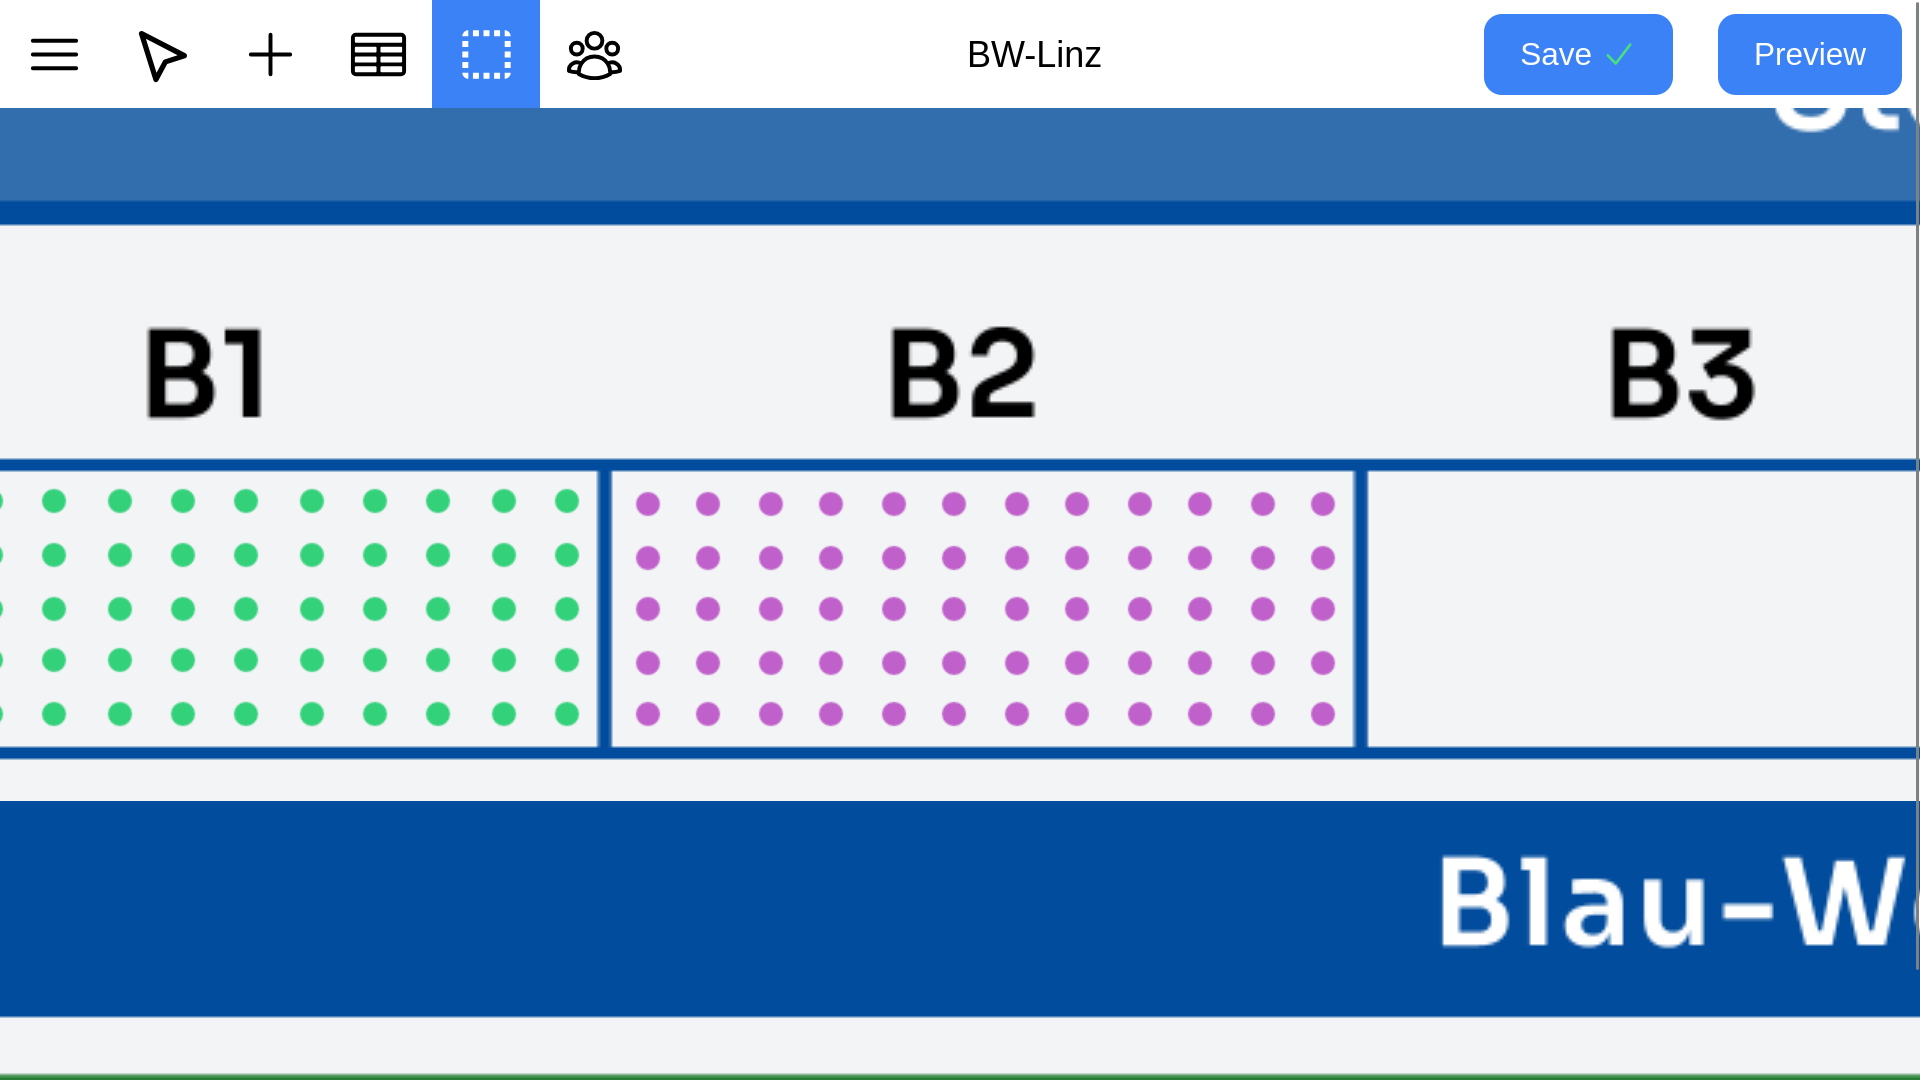
\includegraphics[width=0.4\textwidth]{pics/abstract.png}
    \end{center}
\end{wrapfigure}
SeatGen is a tool developed for Solvistas GmbH to simplify stadium seating plan creation and management. It replaces the inefficient manual process with an intuitive graphical interface, allowing event organizers to design and edit seating layouts without technical expertise.

Built with React, Spring Boot \& Kotlin, and Leaflet.js, SeatGen enables direct seat manipulation, real-time updates, and bulk modifications. This thesis explores the challenges, technologies, and implementation behind SeatGen.
\newpage